% Document layout

\documentclass[a4paper, 12pt]{article}

%Packages

\usepackage{graphicx} % Required for inserting images
\usepackage{fullpage} % Expands text to fill page
\usepackage{amsmath} % For formatting equations
\usepackage{xcolor} % For colors 
\usepackage{float} % For placing images
\usepackage{geometry} % Page dimensions
\usepackage{biblatex} % For bibliographies
\geometry{margin=1in} % Adjusting margin
\usepackage{enumitem} % Controls list environments
\usepackage{parskip}

% Heading: title, author, date

\title{Chemistry Honors Study Guide}
\author{Test 3 S1}
\date{Test date: November 15, 2024}

\begin{document}

\maketitle

\section{LDS Continued}

\subsection*{Definitions}
\begin{itemize}[leftmargin=*, nosep]
    \item \textbf{\textit{resonance:}} The sharing of electrons between multiple bonds, esp. in polyatomic ions.
\end{itemize}

\subsection*{Resonance LDS}

\subsubsection*{Resonance Structures\footnote{https://kpu.pressbooks.pub/organicchemistry/chapter/1-3-resonance-structures/}}
There are many possible resonance structures of one polyatomic anion depending on the number of double bonds needed to cancel out the formal charge on the central atom.
 
Example: \textcolor{blue}{CO$_3$$^{\text{2-}}$ (carbonate)}

\begin{figure}[ht]
    \centering
    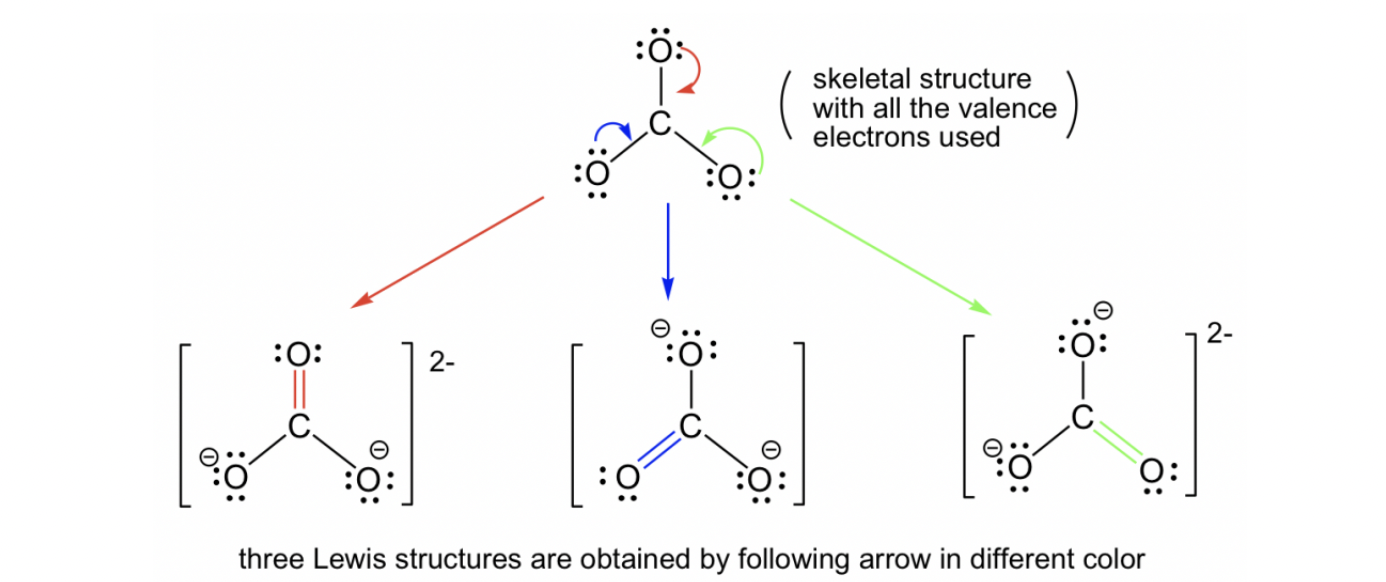
\includegraphics[width=0.8\linewidth]{resonancelds.png}
    \label{fig:200?!}
\end{figure}

\noindent This diagram shows the possibilities of where the double bond could be in carbonate.


\subsubsection*{Combined Resonance Structures\footnote{https://chemfiesta.org/2015/09/18/resonance-structures/}}
In a polyatomic ion, when the central atom has a formal charge of 0, the oxygen atoms around it share their remaining formal charges. A dotted line instead of a bond is drawn from each oxygen atom to the central atom to indicate the shared charge.
 
Example: \textcolor{blue}{NO$_2$$^-$ (nitrite)}

\begin{figure}
    \centering
    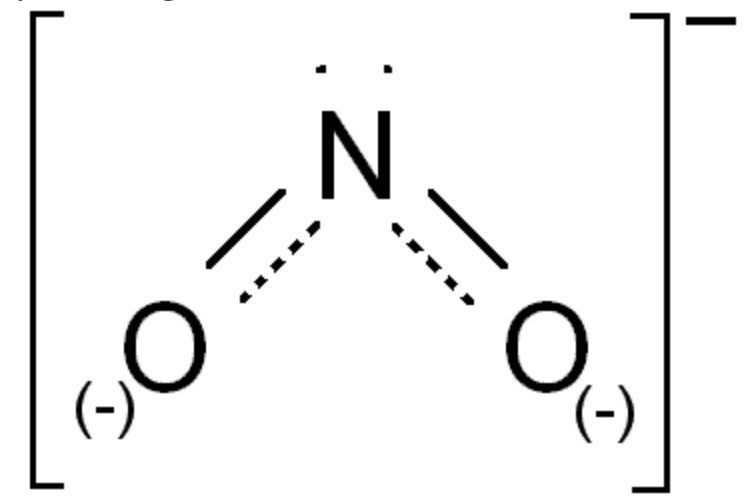
\includegraphics[width=0.3\linewidth]{combinedresonance.png}
    \label{fig:something???}
\end{figure}

\section{Bonding Theories and Geometry}

\subsection*{Definitions}
\begin{itemize}[leftmargin=*, nosep]
    \item \textbf{\textit{molecular orbital:}} An orbital that applies to the entire molecule.
    \item \textbf{\textit{electron domain:}} A distinct region around an atom where lone pair electrons/bonds are found.
    \item \textbf{\textit{pi ($\pi$) bond:}} A type of covalent bond that is a combination of two atomic orbitals overlapping laterally.
    \item \textbf{\textit{sigma ($\sigma$) bond:}} A type of covalent bond that is a combination of two atomic orbitals from end to end. There is exactly one $\sigma$ bond in each single, double, and triple bond (the rest are $\pi$ bonds).
    \item \textbf{\textit{VSEPR (ves-per) theory:}} A model predicting the geometric shape of molecules; stands for \textbf{\underline{V}alence \underline{S}hell \underline{E}lectron \underline{P}air \underline{R}epulsion.}
    \item \textbf{\textit{hybridization:}} The combination of two atomic orbitals to create a new type of hybrid orbital.

\end{itemize}

\subsection*{Molecular Orbitals}

\subsubsection*{$\pi$ Bonding\footnote{https://byjus.com/chemistry/sigma-and-pi-bond/}}

\begin{center}
    Two $p$ orbitals overlap laterally 
\end{center}

\begin{figure}[htbp]
    \centering
    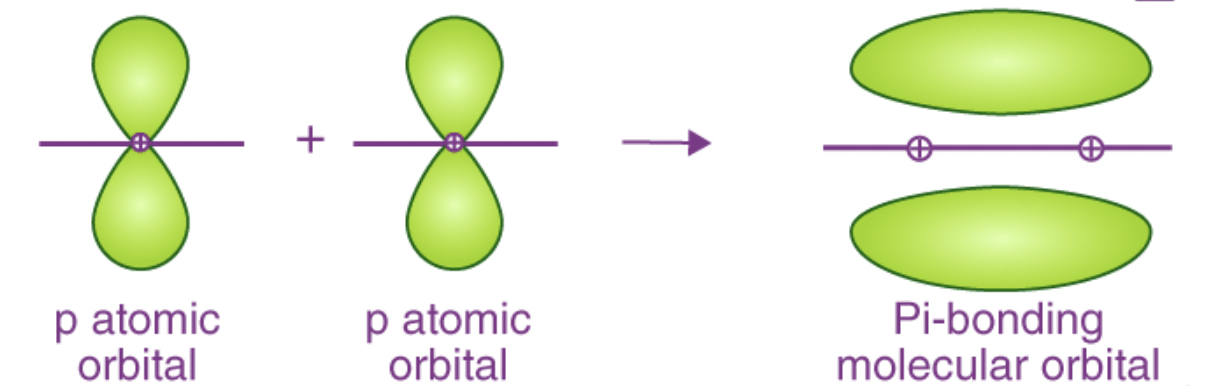
\includegraphics[width=0.5\linewidth]{pibond.png}
    \label{fig:ahhsfhafhshahahdfhoasdf}
\end{figure}

\subsubsection*{$\sigma$ Bonding\footnote{https://www.chemistrylearner.com/sigma-and-pi-bonds.html}}

\begin{center}
    $s$-$s$ overlap (2 half-filled $s$ orbitals)
\end{center}

\begin{figure}[ht]
    \centering
    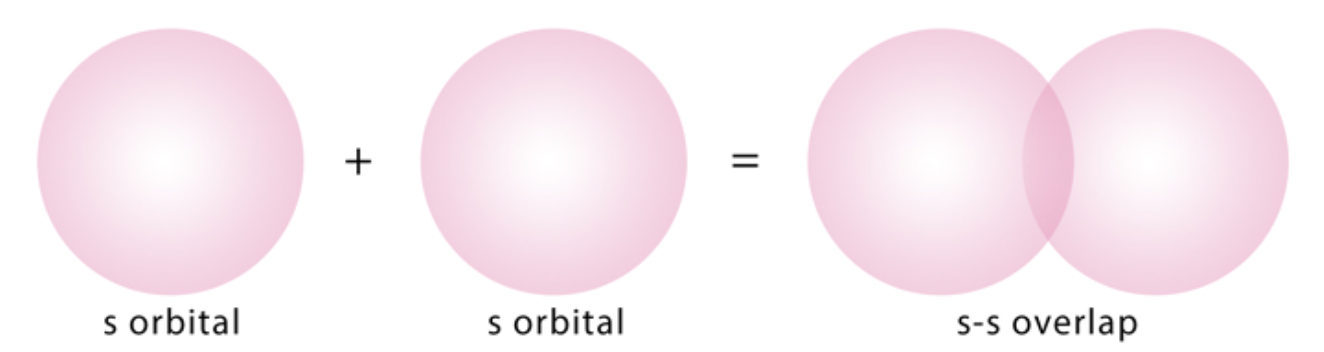
\includegraphics[width=0.45\linewidth]{ssoverlap.png}
    \label{fig:aaaaaaaaaaaaaaaaa}
\end{figure}

\begin{center}
    $s$-$p$ overlap (1 half-filled $s$ orbital and 1 half-filled $p$ orbital)
\end{center}

\begin{figure}[ht]
    \centering
    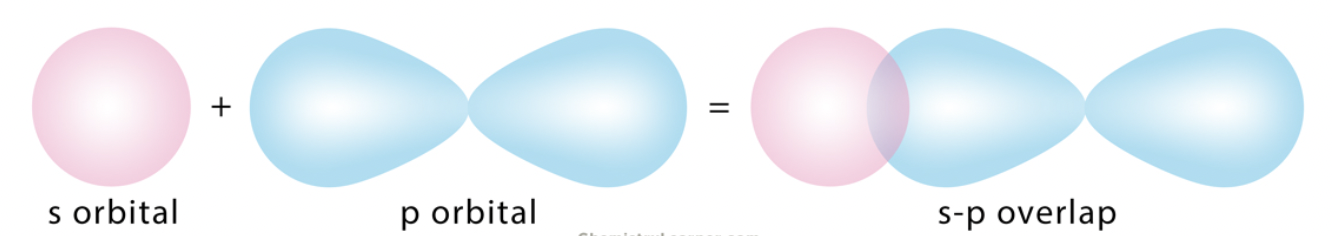
\includegraphics[width=0.5\linewidth]{spoverlap.png}
    \label{fig:enter-label}
\end{figure}

\begin{center}
    $p$-$p$ overlap (2 half-filled $p$ orbitals)
\end{center}

\begin{figure}[ht]
    \centering
    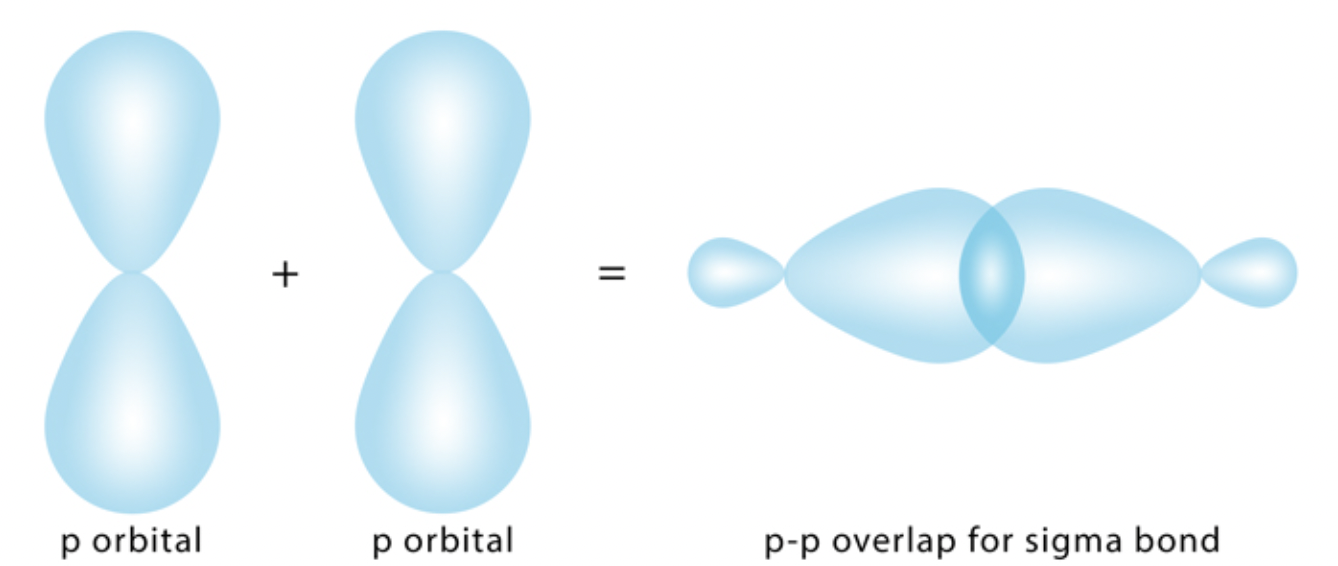
\includegraphics[width=0.45\linewidth]{ppoverlap.png}
    \label{fig:erm}
\end{figure}

\subsection*{Drawing a 3-D Molecule\footnote{https://www.thoughtco.com/wedge-and-dash-projection-definition-602137}}

\begin{itemize}[leftmargin=*, nosep]
    \item line = bond on the plane
    \item 3 lines = bond into the plane
    \item triangle = bond out of the plane
\end{itemize}

\begin{figure}[ht]
    \centering
    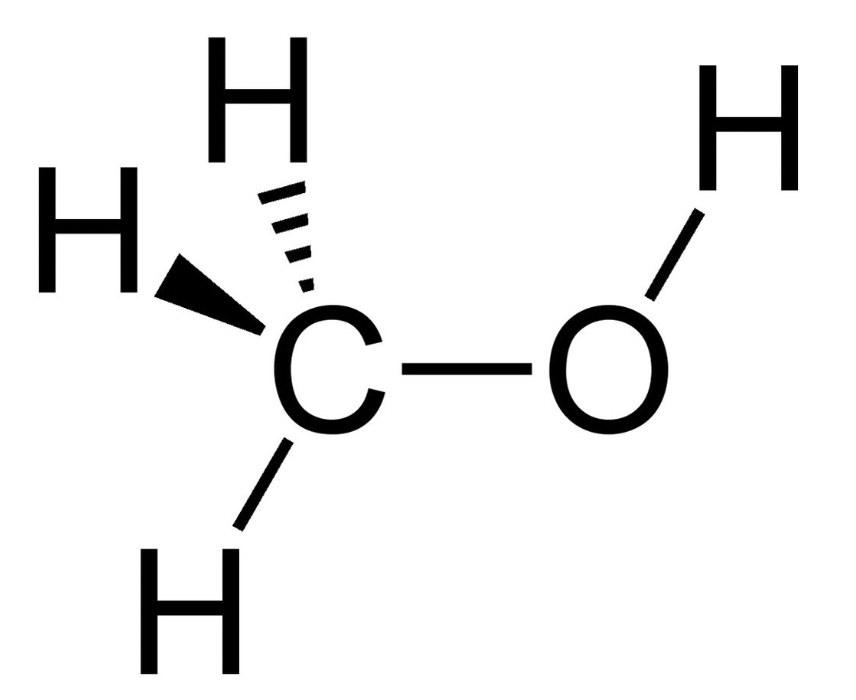
\includegraphics[width=0.4\linewidth]{3dmol.png}
    \label{fig:312456738r902po3iu4}
\end{figure}

\subsection*{VSEPR Theory}
(ed = electron domains; lp = lone pair(s))
\subsubsection*{Electron Geometry}

\begin{centering}

\begin{tabular}{c|c}
    \textbf{\# ed} & \textbf{Name} \\\hline
    2 & \textit{linear} \\
    3 & \textit{trigonal planar} \\
    4 & \textit{tetrahedral} \\
    5 & \textit{trigonal bipyramidal} \\
    6 & \textit{octahedral}
\end{tabular}

\end{centering}

\subsubsection*{Molecular Geometry}
\begin{centering}

\begin{tabular}{c|c|c|c|c|c}
    \textbf{\# ed} & \textbf{0 lp} & \textbf{1 lp} & \textbf{2 lp} & \textbf{3 lp} & \textbf{4 lp} \\\hline
    2 & \textit{linear} & n/a & n/a & n/a & n/a \\
    3 & \textit{trigonal planar} & \textit{bent} & n/a & n/a & n/a \\
    4 & \textit{tetrahedral} & \textit{trigonal pyramidal} & \textit{bent} & n/a & n/a \\
    5 & \textit{trigonal bipyramidal} & \textit{seesaw} & \textit{t-shaped} & \textit{linear} & n/a \\
    6 & \textit{octahedral} & \textit{square pyramidal} & \textit{square planar} & \textit{t-shaped} & \textit{linear}
\end{tabular}

\end{centering}

\subsection*{Hybridization}
(The numbers before the orbital type are the number of that orbital type there are, not the energy level.)
 
$1(s) + 3(p) \xrightarrow{} 4(sp^3)$ (\textbf{tetrahedral} e$^-$ geometry)
\\
$1(s) + 3(p) \xrightarrow{} 3(sp^2) + 1(p)$ (\textbf{trigonal planar} e$^-$ geometry)
\\
$1(s) + 3(p) \xrightarrow{} 2(sp) + 2(p)$ (\textbf{linear} e$^-$ geometry)

\section{Polarity}

\subsection*{Definitions}

\begin{itemize}[leftmargin=*, nosep]
    \item \textbf{\textit{polarity:}} Occurs when one atom attracts electron cloud more than another, therefore making one end more negative.
    \item \textbf{\textit{dipole:}} A pair of separated equal and opposite electric charges.
\end{itemize}

\subsection*{Bond Polarity by Electronegativity}
Polarity is determined by the following equation:

$$\Delta EN = |EN_1 - EN_2| $$

\begin{itemize}[leftmargin=*, nosep]
\item \noindent If $\Delta EN \leq$ 0.4, the particle is \textbf{nonpolar covalent.}
\item If 0.4 $< \Delta EN \leq$ 1.0, the particle is \textbf{moderately polar covalent.}
\item If 1.0 $< \Delta EN \leq$ 2.0, the particle is \textbf{highly polar covalent.}
\item If $< \Delta EN \geq$ 2.0, the particle is \textbf{ionic.}
\end{itemize}

\subsection*{Molecular Polarity}

\begin{itemize}[leftmargin=*, nosep]
    \item If a molecule has no polar bonds, it is not polar.
    \item If a molecule is symmetrical with the same polarity in each bond, it is not polar. (Molecules with linear, trigonal planar, tetrahedral, trigonal bipyramidal, and octahedral molecular geometry and the same element around the central atom are not polar.)
    \item If a molecule contains (a) more electronegative atom(s) on one end than another, the polarity arrow goes in the direction of the electronegative end.
\end{itemize}

\section{Intermolecular Forces (IMFs)}

\subsection*{IMF Types (weakest to strongest)}

\subsubsection*{London Dispersion Forces (LDFs)}
Occur between all molecules. Only IMF between nonpolar molecules

\begin{itemize}[leftmargin=*, nosep]
    \item weakest IMF
    \item attractions between instantaneous dipoles due to moving electrons
    \item also induced dipoles
    \item $\uparrow$ molecule size, polarizability = $\uparrow$ LDF
\end{itemize}

\subsubsection*{Dipole-Dipole Forces (Dip-Dip)}
Formed between polar molecules due to attraction between opposite permanent poles
\textbf{Dipole notation:\footnote{https://byjus.com/chemistry/dipole-moment/}} $\delta^+$ on positive end(s); $\delta^-$ on negative end(s)

\begin{figure}[H]
    \centering
    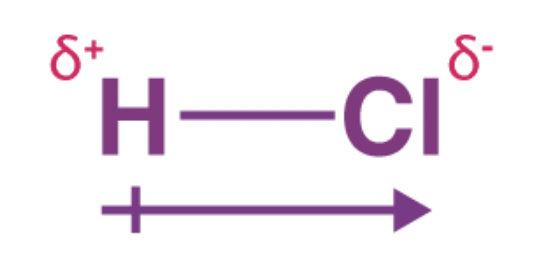
\includegraphics[width=0.3\linewidth]{polarmol.png}
    \label{fig:ummmmmm}
\end{figure}

\subsubsection*{Hydrogen ``Bonding" (H-Bonding)}
Occurs between molecules with N---H, F---H, and O---H bonds. A type of dipole-dipole interaction.

\subsubsection*{Ion-Dipole Interactions}
Formed between ionic compounds and polar compounds.
$$NaCl_{(s)} \longrightarrow Na^+_{(aq)} + Cl^-_{(aq)}$$
Adding salt to water creates a cage effect, increasing density, because molecules are more tightly packed together due to stronger bonds. In order for ionic compounds to dissolve, ion-dipole forces must be stronger than ionic and H bonds.

\subsection*{Macro Effects of IMFs}
$\uparrow$ IMFs = $\uparrow$ boiling point, melting point, surface tension, viscosity
 
\begin{centering}

\begin{tabular}{c|c|c|c}
    \textbf{Name} & \textbf{Formula} & \textbf{Strongest IMF} & \textbf{Boiling Point} \\\hline
    Water & H$_2$O & H-bonds & 100ºC \\
    Methane & CH$_4$ & LDFs & -162ºC \\
    Formaldehyde & CH$_2$O & Dip-dip & -19ºC \\
    Propane & C$_3$H$_8$ & LDFs & -19ºC \\
    Hexane & C$_6$H$_{14}$ & LDFs & 68ºC
\end{tabular}

\end{centering}

\subsubsection*{Trends}
\begin{itemize}[leftmargin=*, nosep]
    \item The relative boiling points of molecules of similar sizes depend on the IMFs present. ($\uparrow$ force = $\uparrow$ b.p.)
    \item The relative boiling points of molecules with the same IMFs depend on the sizes of the molecules. ($\uparrow$ size = $\uparrow$ polarizability = $\uparrow$ b.p.)
\end{itemize}

\subsubsection*{Miscibility}
\textbf{``Like dissolves like"} --- polar + polar and nonpolar + nonpolar are miscible and create a homogeneous mixture; nonpolar + polar are not miscible and create a heterogeneous mixture

\section{Atoms, Molecules, Moles, Grams}

\subsection*{Definitions}

\begin{itemize}[leftmargin=*, nosep]
    \item \textbf{\textit{mole:}} A unit of quantification; 6.02 x 10$^{23}$ (Avogadro's number).
    \item \textbf{\textit{molar mass:}} How many grams a mole of an atom/compound weighs. Units are g/mol.
\end{itemize}

\subsection*{Conversions}

Example: How many \textcolor{blue}{atoms} are in \textcolor{blue}{17 grams} of \textcolor{blue}{MgCl$_2$}?
 
\textcolor{blue}{\textbf{Step 1:} Draw a conversion map.} In order to get from grams to atoms, the steps are as follows:
\\
$$g \longrightarrow mol \longrightarrow {\text{molecules}} \longrightarrow {\text{atoms}}$$
\\
\textcolor{blue}{\textbf{Step 2:} Set up the conversion.} Multiply by the conversion factor(s), (a) unit fraction(s) (equal to 1). Set it up so that the same units cancel out in order to get the desired unit in the end.
\\
$$(17\: g) \times \left(\frac{1 \: mol}{95.211 \: g}\right) \times \left(\frac{6.02 \times 10^{23} \: {\text{molecules}}}{1 \: mol}\right) \times \left(\frac{3 \: {\text{atoms}}}{1 \: {\text{molecules}}}\right)$$
\\
\textcolor{blue}{\textbf{Step 4:} Calculate.} 
\\
$$=3.225 \times 10^{23} \: {\text{atoms}}$$
\\
\textcolor{blue}{\textbf{Step 5:} Check for reasonableness.} 17 grams of MgCl$_2$ should contain a large amount of atoms, which is reflected in the answer.

\subsection*{Percent Composition}
$$\frac{\text{mass of element}}{\text{mass of compound}} \times 100 = \% \: \text{composition}$$
\\
Example: What is the percent composition of iron \textcolor{blue}{(Fe)} in \textcolor{blue}{Fe$_2$O$_3$?}
\\
$$\frac{2(55.85 \: g/mol)}{2(55.85 \: g/mol) + 3(15.999 \: g/mol)} \times 100 = 69.94\%$$


\end{document}

